
\begin{savequote}[8cm]

    We hear a lot these days about genes and molecules, but how does one human brain, or one human being coordinate, or entrain, or resonate with another?  We may not realise it but we live in a world of coordination, at every level and every scale of endeavour.

  \qauthor{--- J. A. S. Kelso  \textit{Coordination and the Complimentary Nature} Presentation to the The New York Academy of Sciences - May 12, 2010}
\end{savequote}


%I do not see any way to avoid the problem of coordination and still understand the physical basis of life.
%\qauthor{--- H. H. Pattee  \textit{The role of instabilities in the evolution of control hierarchies} 1976}


\chapter{\label{chap:theory}A theory of social bonding through joint action}


\minitoc

In response to the knowledge gaps identified in the Introduction, in this chapter I outline a novel theory of social bonding through joint action, which will be tested in subsequent empirical studies of joint action among Chinese rugby players.  While it is now well-established that successful interpersonal entrainment of movement can be responsible for generate positive psychological and social effects, the mechanisms through which entrainment is achieved remain poorly understood.  In particular, I identify team click as a special case phenomenon of joint action and a potential mediator of the relationship between joint action and social bonding in group exercise contexts.  Emerging research from the social cognition of joint action suggests that a continuum of cognitive mechanisms are responsible for establishing and maintaining behavioural coordination between two or more individuals.  More efficient solutions to the cognitive uncertainty of joint action appear to involve reducing the cognitive demands associated with interoceptive predictive modelling and instead increasing reliance on more direct extra-neural coupling with the environment.  These mechanisms also appear to be modulated by inter-individual and cultural variation in knowledge, expertise, experience, and personality type.  Evidence suggests coordination in joint action can set the foundation for social connection, and the phenomenon of team click can be understood as an optimal state of interpersonal coordination in joint action that maximally activates a causal pathway between joint action and social bonding.  I conclude the chapter by summarising a theory of social bonding through joint action, and outlining predictions that arise from this theory.

In this dissertation I attend specifically to the relationship between joint action and social bonding in the group exercise context of professional rugby in China.  In this chapter I formulate a novel theory of social bonding through joint action in order to address the knowledge gaps in the social high theory of group exercise and social bonding.


                                  \begin{CJK}{UTF8}{gbsn}

\section{The development of visceral agency in rugby's newest recruit\label{sect:SHW}}
Sun Hongwei arrived, escorted by his high school athletics coach, to the Beijing Temple of God of Agriculture Institute of Sport (hereafter the Institute) soon after I began my fieldwork in August 2015.  An 18-year-old with a slight build and timid demeanour---his gaze remained diverted to the ground during his first few months at the Institute---Hongwei later told me that he had never seen a rugby ball before that day he arrived.

Hongwei was from Hebei province, immediately surrounding the special prefecture of Beijing, China's capital.  Hongwei's coach had organised a trial for Hongwei with the Beijing Provincial men’s and women's Rugby Program (hereafter the Program) by calling upon social connections to the leadership of the Institute.  Athletes come to the Rugby Program from all over the country.  As I explain in more detail in Chapter ~\ref{chap:researchSetting}, representing Beijing at a provincial level in a sport like rugby can translate into the opportunity to gain entrance to one of China's top universities and enhanced career employment opportunities thereafter.

Rugby is not a popular sport in China, but its recent inclusion in the Olympic games (in the form of the modified seven-a-side version of ``rugby sevens'') means that it now occupies a prominent place in the Chinese sport system.  Rugby programs such as the one at the Institute now exist in 12 of China's 34 provincial level regions, either embedded within, or somehow associated with, tertiary education institutions.  Thus, although rugby and China are not commonly associated terms, rugby now affords Chinese athletes a rare and under-capitalised opportunity to pursue attractive life-course opportunities of education and employment in an intensely competitive education system.

Without exception, the athletes who arrive at the Institute to join the rugby team were not like me; they had not spent their childhoods playing rugby in their schoolyards or watching professional rugby on television. Many who come to rugby transition from other more popular sports such as athletics, basketball, or association football, and often---like Hongwei---have never seen a rugby ball before they arrive.  Most ``start from scratch,'' so to speak, in terms of their grasp of the requirements of the highly interactive and technically complex team sport. In addition to complex patterns of movement coordination, rugby also involves unrestrained body-on-body collisions and intense bouts of high physiological exertion, requiring speed, strength, agility, and endurance to perform all of rugby's technical requirements successfully (see Chapter ~\ref{chap:researchSetting} Section ~\ref{sect:rugbyUnion}).  Learning the game of rugby from a baseline of essentially zero, while also navigating the inevitably demanding social and political dynamics within the team and the Institute, was clearly going to be a daunting task for Hongwei.


                        \begin{center}
                          * * *
                        \end{center}

Hongwei was the first of the Program’s new recruits that I followed closely.  Even compared to other newly arrived junior athletes, he was noticeably timid and shy, particularly in his interactions with the coaches (myself included) and senior players. Nevertheless, Hongwei clearly signalled diligence and commitment through his participation in team activities.  He arrived early to each training session, and carried more than his fair share of the training equipment---a task shared by the most junior members of the team.  Each time I passed Hongwei in the corridors of the Institute he would greet me with a polite bow and greeting, ``Hello Coach'' (\textit{'jiaolian hao'} `教练好').  In these instances, Hongwei would coordinate his greeting with a moment's eye contact, only to return his gaze to the floor and continue walking.

Due to his lack of familiarity with the basic techniques of rugby, Hongwei was initially unable to properly participate in normal training with the rest of the team.  Instead, during the first month or so, Hongwei stood on the sidelines and practiced the basics with other athletes who were unable to fully participate in training due to injury.  He learning how to pass and catch the rugby ball, while stationary and running in-motion.  In my eyes at least---eyes of an observer accustomed to instinctual grasp of these movements from a young age---Hongwei's attempts to accustom himself with the skills of rugby were jarring.  The idiosyncrasies of rugby's ovular ball often foiled Hongwei.  I would regularly see him chasing after a ball on the ground he'd just fumbled, as if he was chasing in vein after a scurrying rabbit tactfully evading his pursuit.

                        \begin{center}
                          * * *
                        \end{center}

I interviewed Hongwei approximately six weeks after he arrived at the Institute.  Hongwei's demeanour during the interview was consistent with the timid and shy one that he presented publicly at training.  As explain below, he did show some signs of captivation with his new sport and social environment.  When I asked about his initial impressions of the on-field demands of rugby, however, Hongwei was quick to confess that he felt utterly unacquainted:

  \begin{quotation}
    SHW: I still haven’t really started to practice any of the team plays or anything; all I can do so far is pass and run a little bit...(but) it's quite fun! \\
    JT: What do you think is the most difficult component of rugby? \\
    SHW: Um\textellipsis well, coordinating with teammates [on the field], particularly coordination in attack.  Because I can't figure it out.  When I first arrived, I didn’t even know what a ``switch play'' or a ``blocker play'' was.
  \end{quotation}

  \begin{quotation}
    SHW: 战术没怎么接触,就是像传球啊、跑动什么的会一点了 \\
    JT: 感觉怎么样?\\
    SHW: 挺好玩的!\\
    JT: 你认为橄榄球最难的一部分是什么? \\
    SHW: ...打配合,进攻的配合,因为搞不明白,刚来的时候也不知道什么交叉,后插什么的 \\
  \end{quotation}

Hongwei was self-critical in this confession regarding his minimal grasp of the technical requirements of joint action in rugby.  The obvious stress and anxiety he expressed was indicative of a broader trend with the other athletes I interviewed, as I will explain in more detail in the ethnographic sections of this dissertation (see Chapters ~\ref{chap:ethnoField} \nobreakdash~\ref{chap:ethnoResults}). When athletes were asked in interviews about the most difficult aspect of rugby, on-field coordination with teammates was by far the most common answer, particularly among the new recruits and most junior athletes.

As I directed the interview towards topics beyond the on-field technical demands of rugby, Hongwei was more positive, framing rugby as an exciting new opportunity, and commenting that his friends and family were in awe of the fact that he is playing such an impressively ``strong'' physical sport like rugby.  When I asked him about something new that he had learnt through playing rugby, Hongwei automatically responded by emphasising the social dimensions to his experience at the Institute:

  \begin{quotation}
    ``...I think it's mainly this thing of having teammates. Before, when I was training for an individual sport, it was just me training by myself. [In that environment] it was a case of whoever trained well was successful.  But now with this team of brothers, elder teammates will take care of younger teammates. We all train together, and if you can’t do something, you can always ask your elder teammates...[Rugby] is so much better, because in an individual sport, if you can't master something, you have to go to your coach for help. Other athletes don't want to teach you, because if you surpass them, then they have to work even harder to keep up... I have had to learn about helping others, because rugby is not like an individual sport, where you look after your own performance and that's it.  In a team sport, if you don't do well, there's no need to get too frustrated or upset, because other athletes will help you out, and I will also help others out, that type of collaboration with each other.''
  \end{quotation}

\begin{CJK}{UTF8}{gbsn}
  \begin{quotation}
    我觉得主要是师哥师弟的这一块儿,原来练个体项目都是自己练自己的,谁练好了谁厉害,但是现在师哥师弟,有师哥照顾师弟带着,互相练,我不会我可以问师哥
    ...因为个人项目你不会就必须要找教练,但是别人不愿意教你,因为你把别人超越了那别人还还得努力。 学到互相帮助,因为向个体项目自己成绩自己来拿就行,而像团体项目,即使自己做不好,也不用太泄气太沮丧,因为别人会帮你做好,我也会帮别人做好,互相协作的那种.
  \end{quotation}
\end{CJK}

Hongwei's explicit reference to the collegiality of the team, and his position as junior member, highlights that the technical skills of rugby were not the only novel components of his experience.  Hongwei's background was in track and field (his event was pentathlon, very much an individual sport), and the team environment was completely new to him.  This was also the case for many of the other athletes in the team.  As I listened to his experiences associating rugby and group membership, I could not help but associate the quality of these declarations of prosociality with his overly mechanical imitation of rugby's foundational techniques.  In both I saw his willingness and desire to signal commitment; but both lacked a certain grasp or command that one would expect from an athlete more habituated to rugby.

                            \begin{center}
                              * * *
                            \end{center}

A few months passed, and Hongwei continued to train.  He was as eager and committed as when he began, and I did notice some gradual improvement in his grasp of rugby's basic skills.  But he also remained extremely reserved, keeping his head low at all times in team settings, unless addressed by senior players or coaches.

Then, one evening when I had returned to my room in the Institute dormitory from a three-week hiatus in Australia over Christmas of 2015, I heard a knock on my open door, and to my surprise Hongwei took an assertive stride into my room, carrying in two arms a draw-string bag containing rugby balls (which were in need of more air before the next day's training session).  Hongwei had never ventured into my room before, apart from our first interview two months earlier---but certainly never on his own accord.  Remarkably, Hongwei looked me straight in the eyes with his head held high and energy beaming from his face and chest.  I couldn't help but smile and ask, with genuine intrigue, ``How have you found training recently?''
``Very good'' he said, assertively and excitedly.  ``Much better than before.  At least now I know what’s going on at training, I can keep up with the plays!''  A big smile grew on his face as he continued to hold my gaze.  ``Oh good!'' I said, a little bit shocked.  I congratulated him for his hard work in training while I had been away, and encouraged him to keep at it.  Wow, I remember thinking to myself, Hongwei was all of a sudden possessed by a powerful force.  Somehow, his adherence to rugby had instiled him with a visceral sense of agency.

                          \begin{center}
                            * * *
                          \end{center}

In the same way that Adrian's opening monologue (Chapter ~\ref{chap:intro} Section ~\ref{sect:adrian}) suggested a relationship between the on-field dimensions of rugby and social processes between teammates, the fact that aspects of Hongwei's personal and social demeanour at the Institute appeared to covary with his familiarity with the technical requirements of rugby over time suggests a relationship between joint action and group membership that is worthy of further investigation.
%HW's change is a change in attitude (Bateson) agency

How is it possible to scientifically account for the unmistakably ``visceral'' quality of Hongwei's transformation from timid newcomer to budding Beijing rugby player?  How can these ethnographic observations be explained in terms of generalisable cognitive mechanisms and systems dynamics of joint action?  Finally, and ultimately, how do answers to these questions improve our ability to comprehend the evolutionary significance of group exercise in the human record?



\section{The need for a theory of joint action and social bonding in group exercise}

Physical movement is central to the adaptive success of biological life, particularly life which can intentionally direct movement in order to bring about change in the environment.  Humans display a rich capacity for complex forms of autonomic and preconceived physical movement, which is employed both when coordinating behaviours with the environment and socially with conspecifics.  The ability of humans to coordinate movement with one another vastly increases the range of their potential actions, and is a fundamental explanation for our species' evolutionary success \citep{Tomasello2009}.  Scientific understandings of the precise details concerning how humans move together, and why joint action may be crucial to the human evolutionary niche, remain rudimentary.  In this chapter, I propose that a more thorough understanding of mechanisms and dynamics of interpersonal coordination of physical movement could help develop cognitive and evolutionary explanations for group exercise.

As discussed in the introductory chapter, current evidence detailing the proximate mechanisms of group exercise suggests a relationship between group exercise and social bonding, whereby 1) sustained moderate intensity physiological exertion and 2) behavioural synchrony and 2) are responsible for generating a psychophysiological environment conducive to social affiliation and trust (see Chapter ~\ref{chap:intro} Section ~\ref{sect:socialHigh} for a more thorough explanation).  This proximate evidence lends support to the hypothesis that group activities involving coordinated movement and physiological exertion, such as those found in ritual, music, dance, and sport, have been favoured in evolutionary processes of cultural group selection, owing to the fact that they promote social cohesion \cite{Dunbar2010}, along with other individual-level adaptive benefits \citep{Cohen2017}.

Beyond moderate intensity exertion, behavioural synchrony, and a feel-good social high, many identifiable empirical aspects of the phenomenon of group exercise remain unaccounted for by the social high theory.  Some group exercise contexts involve extreme physiological cost (i.e., anaerobic exertion, pain, violence), complex multilayered joint action, and---associated with these dimensions---subjective experiences of profound meaning and ``team click.''  The prevalence of these under-appreciated dimensions of group exercise suggests the possibility of additional causal pathways between group exercise and social bonding.  The sport of rugby union (the specific empirical focus of this dissertation) serves as an illustration of these putative causal pathways in action.  A framework that theorises additional explanatory mechanisms is required in order to test these relationships.

In this chapter, I develop a theory of joint action and social bonding that reaches beyond behavioural synchrony as a stand-in for successful joint action.  As explained in the previous chapter, behavioural synchrony is an obvious place to begin an investigation into the social effects and evolutionary significance of group exercise (see Chapter ~\ref{chap:intro} Section ~\ref{sect:pathBeyondSynch}). Fixation on strict synchrony as a stand-in for successful coordination in joint action, however, threatens to occlude important proximate mechanisms and psychological effects of interpersonal coordination in joint action.

The embodied and dynamic nature of

In particular, I focus on the widely observable phenomenon of ``team
click'' in complex multilayered joint action.  Team click entails the pleasurable experience of flow in joint action, tacit understanding and reliability between co-actors, a blurring of agency between self and team, and an atmosphere or aura surrounding the team.  Team click entails the operation of neurocognitive mechanisms of anticipation, monitoring, and adaptation, as well as emotional (interoceptive) mechanisms of appraisal and motivation.  Importantly, team click is also often reported as a surprising or unanticipated event. While team click is an ideal state of joint action, it always appears to come somewhat as a surprise.

I use the prevailing cognitive theory of ``active inference'' \citep{Friston2010} to conceptualise joint action as a dynamical process in which prediction, perception, action, and emotion, are functionally integrated in the ultimate pursuit of minimising free energy in the task-specific environment \citep{Clark2015}.  Using this theoretical conception, individuals can be seen to flexibly deploy a range of cognitive strategies in order to establish and sustain coordination in joint action.  Rather than being bound to ``either/or'' choices between fast or slow, habitual or mental, emotional or cognitive cognitive responses \citep[cf.][]{Kahneman2011}, the active inference paradigm can account for the preference for efficiency, the need for flexibility, and the unrelenting drive for novelty displayed by processes of human cognition \citep{Friston2011}.

%This would make sense in the case of group exercise context such as rugby, which involve high levels of uncertainty and in the moment joint action: in these contexts interoceptive signals would be given higher precision weights (what is anticipated is more limited to the immediate body and its surrounds); click arrives from outside

An active conception of human cognition opens up a space for testable predictions concerning the relationship between joint action, team click, and social bonding.  I predict a positive relationship between 1) joint action and team click, and 2) team click and social bonding.  I also predict that 3) team click will mediate a direct relationship between joint action and social bonding. In addition to these core predictions, I accommodate for the role of cultural and individual variation in shaping and constraining patterns of behaviour.

In this chapter, I begin by introducing the phenomenon of team click.  I then introduce the paradigm of active inference, including the key theoretical building blocks required for this the theory.  With this theoretical framework established, I justify the predicted relationships between 1) joint action and team click, as well as 2) team click and social bonding.  Finally, I summarise a novel theory of social bonding through joint action, and outline the specific predictions of the theory.



\section{Human solutions to the challenge of joint action}
\subsection{The degrees of freedom problem and its solutions in human movement\label{sect:dfProblem}}

\textcite{Bernstein1967} was the first to point out the astounding computational challenge associated with coordinated physical movement in multi-component living systems.  In the case of human intra-personal movement, for example, an impressive balance is somehow struct between flexibility, precision, and control, whereby hundreds of muscles and joints coordinate to perform many different tasks of everyday life.  When we grasp a cup or catch a ball, many individual muscles and joints---each with their degrees of freedom---work together in fine concert.  Bernstein found it unlikely, from a computational perspective, that the central nervous system would be able to finely control all the possible movements (the degrees of freedom) of each single muscle individually to create coherently directed movements---it would be computationally impossible. Rather, he suggested that muscles and joints form  ``functional synergies''---flexible function-specific self-organising assemblies---by locally coupling and constraining each other’s degrees of freedom to greatly reduce the amount of control needed (more on this below in Section ~\ref{}).

Intra-personal and interpersonal human movement both rely on the nervous system’s capacity to anticipate, attend, and adapt to the conditions of the environment \citep{Keller2014}.  In the case of intra-personal human movement, successful coordination of is made possible by the nervous system's direct access to information concerning the spatiotemporal position of the body and its relationship to the environment.  Privileged access to this information enables habituated coupling of movement control system to the organism's various degrees of freedom, and therefore the emergence of self-organisng functional synergies.

By contrast, interpersonal movement coordination poses a much more significant challenge.  In the case of interpersonal coordination, the combination of 1) limited reliability of sensory modalities as a source of information about the action of others \citep{Wilson2005,Wolpert2003,Frith2007} and 2) the informational complexity associated with a cognitive system comprising multiple autonomous agents \citep{Bernstein1967} means that successful coordination in joint action is an inherently difficult and highly improbable cognitive challenge.  How exactly do humans face up to this cognitive challenge, and, quite often, successfully surmount it?

An answer to this question requires close attention to the various sophisticated cognitive, behavioural, and cultural capacities that define human's species-unique evolutionary niche \citep{Roepstorff2010,Clark2015,Fuentes2016}. Our ability for technical manipulation of extra-somatic materials and ecologies; advanced theory of mind; and information-rich, malleable, and scalable communication systems affords complex behavioural repertoires involving that enable interaction between groups as small as two and conceivably as large as two million \citep{Nowak2017}.  In this dissertation I focus on interpersonal coordination of physical movement as a basal layer to human social interaction that towers many layers of complexity.

\textcite{Vesper2010}, building on previous work by  \textcite{Sebanz2006}, has proposed a minimal architecture for joint action.  The minimal architecture of joint action requires that individuals:

\begin{enumerate}
  \item Represent a shared goal, as well as representing one’s own individual contribution to the shared goal.
  \item Apply monitoring and prediction processes to each partner’s actions. This includes monitoring the extent to which shared goals or tasks are being fulfilled while at the same time predicting a partner’s actions.
  \item Facilitate continuous coordination via coordination smoothing, defined as the process of continuously improving one’s prediction of the partner’s action.
\end{enumerate}

Based on current understandings of human cognition motor control, it is unlikely that solutions to these minimal requirements of joint action could be driven solely by central, executive control processes in the central nervous system---joint action would be too slow and costly.  It is similarly unlikely that processes of unconstrained automatic alignment (with no higher-level coordination) could possibly enable joint action---joint action would be too undirected and chaotic \citep{Fusaroli2014}.  Rather, it seems more plausible that joint action is facilitated by a continuum of mechanisms spanning executive control through to direct coupling.  To establish and sustain interpersonal coordination, participants selectively recruit multiple behaviours and processes, which in turn become more interdependent and constrained by the function of the ongoing activity.

Importantly, it appears that successful coordination of behaviour in joint action is rewarded in the form of powerful psychophysiological states of arousal, euphoria, and eudemonic wellbeing.  Thus, while joint action is daunting and improbable from a cognitive perspective, it is also clear that humans have devised mechanisms through which successful joint action is rewarded. The relationship between complex coordination in joint action and team click suggests that successful coordination in joint action could activate a pathway to social bonding.  In the section below, I outline the phenomenon of team click, and point to evidence of its connection to mechanisms of joint action and social bonding.


\section{Introducing the phenomenon of team click\label{sect:teamClickIntro}}

One of the big mysteries of competitive team sport, particularly at the elite level, is the elusiveness of peak team performance.  While each individual athlete may exhibit expert level competence in sport specific skills, the much sought after aggregation of these components, i.e., a team that consistently performs ``in the zone,'' and ``firing on all cylinders,'' in reality often proves frustratingly difficult to achieve and sustain.  As King and De Rond \textcite[568]{King2011} note in their ethnography of the 2008 Cambridge University rowing crew who participated (and who were eventually victorious) in the famous annual Boat Race against Oxford University, the search for collective rhythm is a universal in human social interaction, but  the physiological and psychological complexity of finding that rhythm ``...is extremely difficult to attain; collective performance is a possibility not a certainty.''   The moment in which everything ``clicks'' into place in team sport can, for various reasons, disappear as abruptly as it arrives, if indeed it arrives at all.

But, when team click is somehow cultivated, and even sustained, it is celebrated as the ultimate, albeit often inexplicable magic of sporting feats. Consider Leicester City Football Club's unbelievable outhouse-to-penthouse title run in the 2015 English Premier League, the recent dominance of the Golden State Warriors in the American National Basketball League, or the astonishingly consistent performance of the New Zealand men's national rugby union team (the ``All Blacks'').
    \footnote{The All Blacks are arguably the most successful sporting team ever, with a winning percentage of 77\% in the last 150 years (and 88\% in the last 6 years) \citep{Kerr2013}}.
All of these successful teams carry with them a powerful ``aura'' associated with their capacity to effectively coordinate their behaviours on the field over extended time scales: individual games, seasons, and, in the case of the All Blacks, entire generations.  The aura associated with such rare instances of collective performance can seduce fascination and elaborate exegesis.

    %In this thesis I commit to the more banal task of naturalising the phenomenon of team click, by locating it within a novel theory of social bonding through joint action.

    For the purposes of this dissertation, I use the term team click to describe the phenomenology of peak performance within a team of athlete engaged in joint action, but the term has potentially broader applications beyond group exercise.  For athletes, coaches, and spectators alike, team click can be a hugely powerful sensation.  As theologian Michael Novak explains, ``[f]or those who have participated on a team that has known the click of communality, the experience is unforgettable, like that of having attained, for a while at least, a higher level of existence'' \citep[11]{White2011}.  It has been extensively documented in the psychological literature of flow and optimal human performance in sport that athletes engaged in team coordination often report total absorption in and complete focus on the task at hand, a transformation of the experience of time (either speeding up or slowing down), and a blurring or transcendence of individual agency, or a ``loss of self''   \citep{Csikszentmihalyi1992,Jackson1995,Jackson1999,McNeill1995}.  Research suggests that flow often occurs in scenarios in which there are clear goals inherent in the activity, as well as unambiguous feedback concerning extent to which goals are either being achieved or not.  In addition, scenarios most conducive to the experience of flow are those in which the technical requirements are challenging but achievable if practitioners are able to extend slightly beyond their normal capabilities\citep{Fong2015}.
    The coalescence of these factors is intrinsically rewarding and autotelic\citep{Csikszentmihalyi1975}, activating both ``hedonic'' and ``eudaimonic'' dimensions of subjective well-being \citep{Huta2010,Fave2009}.


    %It was just one of those programs that clicked. I mean everything went right, everything felt good . . . it’s just such a rush, like you feel it could go on and on and on, like you don’t want it to stop because it’s going so well. It’s almost as though you don’t have to think, it’s like everything goes automatically without thinking . . . it’s like you’re in automatic pilot, so you don‘t have any thoughts. You hear the music but you’re not aware that you’re hearing it, because it’s a part of it alI.

    The experience of flow has by now been extensively studied by psychologists and neuroscientists, from which a series of neuropharmacological \citep{Boecker2008}, neurocognitive \citep{Dietrich2006,Dietrich2011,Labelle2013}, and psychological \citep{Csikszentmihalyi1992} theories for its emergence have been tabled.  The vast majority of flow research has focussed on the experience of the individual---the athlete, musician, or performer.  Some attempts have been made to extended an analysis of flow and its antecedents to the level of the group and dynamics of interpersonal coordination---a phenomenon termed ``group flow'' \citep{Sawyer2006}---but these attempts lack coherence and development.

    Team click shares many similarities with the psychological states associated with flow, but is distinct in that it specifically delineates perceptions of joint action from individual action, and therefore implicates physiological, cognitive, and social mechanisms unique to joint action \citep{Vesper2010}, including the complexity systems dynamics associated with participating in a socially-coordinated, multi-agent system of physical movement \citep{Kelso2009}.  Team click is anecdotally present in a wide range of joint action contexts, and is often associated in these contexts with psychological processes of positive affect and wellbeing, as well as personal agency, social affiliation, and group membership \citep{Jackson1995,Marsh2009,Wheatley2012,Slingerland2014}.

    In the 1990s, psychologist Susan Jackson conducted a number of qualitative studies documenting athletes' (in this case elite figure skaters) experience of flow in solo and joint action:

    \begin{quotation}
      What was really so special about this performance was that there was nothing between (partner's name) and I but flow.  You know, through the whole three minutes.  That meant that her mind and my mind were clear and in the same...in a partnership. It’s always adjustments for ``Am I?'' and ``Are You?'' and ``Where Are We?'' and stuff like that.  That day was really a marriage of (partner) and (self) and the ice.  So I think it’s a different kind of flow experience than a single skater who has much more control over themselves. \citep[173-4]{Jackson1992}.
    \end{quotation}

    This passage, taken from an interview with a professional figure skater, demonstrates the key elements of distinction between the experience of ``click'' in solo and joint action.  As explained in Section ~\ref{sect:JAbeyondSync}, joint action requires constant finessing (adjustments) of behaviours and intentions between co-participants in which individuals are consulting internal models of self, other, and joint action \citep{Pesquita2017}. This passage thus highlights the cognitive complexity of joint over individual action, suggesting the cost and uncertainty associated with attending to and attempting to control the movement df of others in addition to one's own.  ``Click'' in joint action, by contrast, may represent jitter-less ``co-confidence'' in which fixation on the contributions of you and I are momentarily abandoned or down regulated, and the agency of ``we'' is realised \citep{Gallotti2013,Noy2017}.

    Importantly, team click appears to have important flow-on consequences relevant to social bonding and affiliation. Tightly synchronised activity in particular, found in team sports such as rowing, can help dissolve the boundaries between individual and social agency: ``In rowing...it feels like you have at your command the power of everybody else in the boat. You are exponentially magnified. What was a strain before becomes easier. It is absolutely the ultimate team sport'' \citep{Brown2016}.
    The blurring of agency between self and team may be responsible for facilitating affiliation and trust between teammates in competitive athletic environments such as professional rugby, which often involves high physiological stress and uncertainty.  As Jeremy Paul, a famous Australian Rugby player commented of his late teammate Dan Vickerman ``...you always wanted a guy who would go into the trenches with you and he always played consistently well...he could really play and was just one of the good lads that you enjoyed his company'' \citep{Fox-Sports2017}.  In this sense, the experience of team click may act as a social diagnostic tool, a powerful signal of commitment to joint action and willingness to cooperate \citep{Reddish2013a}. \\
    \\
    \\

    \noindent\fbox{%
        \parbox{\textwidth}{%
    Team click refers to the perception of peak team performance.  Based on anecdote and evidence from psychology and anthropology, an individual's perception of team click should contain some or all of the following components:
        \begin{enumerate}
          \item Flow or coherence of joint action
          \item Tacit understanding between co-actors
          \item Atmosphere or aura around team performance
          \item Teammates are responsible for extending individual ability
          \item Teammates are reliable co-actors
          \item The individual is a reliable co-actor for teammates
        \end{enumerate}
        }%
    }

    \\
    \\
    \\

    %SURPRISING:
    %Oh, it’s awesome! Everything’s at peace . . . the crowd was involved, we were involved as a pair team, and we were just aware of everything, it just kept snowballing, like we weren’t going to miss, and it was great, it was an awesome experience.


    As summarised above, team click is a phenomenon distinct to joint action.  Team click involves an experience of pleasurable flow or coherence of joint action, tacit (rather than explicit) understanding between co-participants, a degree of aura or positivity around joint action, a blurring of agency between self, other and group (or ``we''), and perception of reliability of others and self in performing their roles. Importantly, team click derives from instances of joint action defined more broadly than exact behavioural synchrony. Team click thus offers a powerful empirical anchor for exploring a broader relationship between joint action and social bonding in group exercise contexts.  In the sections that follow, I outline the building blocks necessary to formulate a novel theory of social bonding through joint action. Within this theory, team click is proposed as a mediating construct, through which the bonding effects of joint action are maximised.


\section{Active Inference \label{sect:activeIn}}

Real-word instances of group exercise are complex and multidimensional behavioural phenomena involving dynamic interaction of multiple brains and bodies, situated in varied and richly resourced cultural ecologies.  Development of cognitive and evolutionary theories that can account for this complexity, and in so doing reconcile some of the identifiable gaps in existing accounts, remains a work in progress \citep{Fuentes2016}.  Team click is a salient and widely identifiable phenomenon that is useful as an anchor for empirically grounding a theory of joint action and social bonding in group exericse.

Researchers have pointed out that flow---a concept that shares many similarities with team click---has traditionally escaped rigorous scientific analysis \citep{Dietrich2010a,Slingerland2014}.  Dietrich, for example, explains that flow presents a paradox that is difficult to explain according to traditional theories of attention and mental effort, which tend to assume better performance, on any task, is associated with increased conscious effort allocated to that task \citep{Dietrich2004b}.  Flow appears to entail spectrum of both effortful and seemingly effortless cognitions implicating embodied action and the resources of the bio-external environment.  Team click, too, is a multidimensional process involving mental, embodied, emotional, and social dimensions.  Equipped with only rudimentary explanatory tools from a youthful science of the human mind (cognitive science), it is understandable that scientific progress on the topic has been gradual.

A long-standing movement within the cognitive and behavioural sciences has called for a greater recognition of the physical and dynamical properties of information transfer and coordination within biological systems.  Proponents of so-called embodied, embedded, enactive or extended cognition \citep[now collectively referred to as ``4E cognition,'' see][]{Menary2010}, emphasise that cognition typically involves acting with a physical body on an environment in which that body is immersed. Researchers in this movement call out traditional models of human cognition for being too static, abstract, and compartmentalised: human behaviour is traditionally rendered as the outcome of a linear chain of perception, a-modal representation, and action-selection, located discretely either within the brain or else within certain (often dualistic) subsystems of the brain ( \citep[e.g., emotional and cognitive, System 1 (fast) and System 2 (slow), implicit and explicit, and so on; cf.][]{Diennes1999,Kahneman2011}.

The core of the 4E argument can be boiled down to the idea that just as humans physically move, so too does the information that supports human movement (cognition).  Human inferential processes not only activate physical movement, but are also activated by movement, in a dynamical loop of reciprocal causation.  While proponents of the 4E approach have made valuable contributions to a definition of what traditional theories of human cognition are \textit{not}, empirical evidence capable of adjudicating between testable hypotheses has lagged behind high-volume and high-postured debate.  Interestingly, the debate over the nature of cognition shares many properties with a similar debate over the nature of evolutionary change \citep{Nowak2010,Scott-Phillips2011,Laland2014,Fuentes2016}.

%\subsection{An ``active'' theoretical solution}
A paradigm shift in cognitive and behavioural sciences is shedding new light on human solutions to the challenge of joint action.  Recent advances in neuroimaging technologies \citep{Frith2007}, neurocomputational theories of brain function \citep{Friston2010,Frith2010,Yufik2013,Clark2013}, and constructive attempts to extend the theoretical paradigm of human social cognition to account for inter-individual processes of interaction and coordination \citep{Sebanz2006,Dale2014}, have resulted in a theoretical paradigm, in which it is now more clearly understood that cognitive processes relevant to joint action are distributed throughout brains, bodies, and the physical environment of the ecological niche in which they are situated.  As I explain below, this shift in understanding of human cognition allows for a more powerful and fine-grained explanatory model of how joint action---and, in turn, social connection---could achieved between two or more participants.


\subsection{Thermodynamic cognition\label{sect:thermoCog}}

The paradigm of active inference has its roots in conception of human cognition that adheres to the thermodynamic constraints of living systems \citep{Carhart-Harris2014,Yufik2017}.  The laws of thermodynamics delineate the behaviour of all systems involving matter and energy.  In particular, the Second Law of Thermodynamics suggests that all such systems are subject to entropy---the tendency of a closed system to dissipate toward an equilibrium state of disorder or chaos \citep{Wolfram2002}.  For biological systems, life itself can be represented as the ongoing process of minimising or negating entropy by maintaining an equilibrium of internal order distanced from the external equilibrium of disorder \citep{Schrödinger1944}.  The current claim is that the human brain---a ``measure-preserving dynamical system''---is no exception to the Second Law, and that the processes of information transfer (cognition) performed by human brains will in some ultimate sense adhere to the management of physical and information-theoretic entropy in an organism's exchanges with the environment \citep{Yufik2002,Yufik2013,Friston2010Sengupta2013,Sengupta2016,Sengupta2017}.

Efficient regulation of living systems requires mechanisms that incorporate models of the system and its relation to environment \citep{Conant1970}.  While primitive animals possess small repertoires of genetically fixed, rigid models, more advanced animals possess larger and more flexible repertoires that are amenable to experience-driven modifications.  Both genetically fixed and experience-driven modifications are forms of learning: models are sculpted by external feedback conveying statistical properties of the environment \citep{Yufik2013}.  In humans, implicit models become responsive to self-directed composition and modification based on ``interoceptive'' (stimuli produced within the organism), as opposed (or in addition) to ``exteroceptive'' (stimuli that are external to an organism) feedback \citep{Yufik1998}.

Constructing and manipulating models of sensory inputs can be seen as a means for reaching thermodynamic efficiency in the human brain \citep{Yufik2013}. However, constructing and correcting models consumes energy.  Thus, successful models that persist without or with minimal correction yield the double benefit of reducing internal energy consumption while also optimising (increasing or stabilising) external inflows of energy (or information).  Within this paradigm, thermodynamic ``free energy'' is used as a measure of the energy available to a system to do useful ``work'' at any given time \citep[and entropy is the long-term average of free energy, see][]{Stoner2000,Friston2013}.  In the case of living systems, free energy enables work that contributes to the organismic regulation with the environment. The better the model fit, the lower the free energy, or in other words, more of the system's resources are being put to effective work in representing the world.  It has been suggested that evolution obtains progressively more efficient mechanisms for detecting and exploiting free energy deposits, culminating in consciousness, which resembles the successful integration of various neural networks for coherent consumption of free energy \citep{Annila2016}.

In summary, the emerging paradigm of thermodynamic cognition suggests that humans' behavioural interactions with the environment are constrained by the mandate, common to all multi-component living systems, of free energy minimisation \citep{Friston2013}.  As I explain below, this mandate has important implications for predictions about human behaviour, particularly in the case of social behaviour.

The overarching theoretical framework of thermodynamic cognition is thus important as a starting point for understanding the diverse range of component mechanisms and coordination dynamics that enable joint action, as well as the psychological and social effects of participation in joint action, including the phenomenon of team click.

%Cognition: information into understanding and ``grasp''
%Internal order can be produced by gradients of energy (matter/energy) flows through living systems. Structures so produced help not only draw more energy through the system, lengthen its retention time in the system, but also dissipate degraded energy, or entropy, to the environment. Living systems then are seen an instance of a more general phenomena of dissipative structures.

\subsubsection{Predictive coding}
Research suggests that models capable of maintaining organismic regulation with the environment (i.e., by reducing free energy) must be able to anticipate sensory inputs before they occur. As Pickering and Clark explain, ``predictions can power learning, help finesse time delays, and enable a suite of potent capacities for motor imagination and simulation-based reasoning'' \citep[6]{Pickering2014}.  Currently, all enduring theoretical models of human cognition and motor control generally agree that prediction is crucial for effective behaviour: in order to act effectively in the world, the brain generates ``forward models'' that anticipate perceptual inputs and desired motor states \citep{Pickering2014}.  Disagreement has emerged, however, in relation to the neurocomputational architecture that delivers forward models.  The original paradigmatic theory of motor control suggested that forward models for action relied on special-purpose mechanism \textit{auxiliary} to core mechanisms of perception of action \citep{Wolpert1997}.  A more recent alternative proposal suggests that forward models, instead of being auxiliary to, may instead lie at the heart of, all forms of perception and action \citep{Friston2010}.  In the ``predictive coding'' \citep{Rao1999} or ``predictive processing'' account \citep{Clark2013}, processes of prediction are \textit{integrated} into perception and action itself, offering a more efficient and embodied conception of human cognition (for a more detailed review of Auxiliary Forward Models and Integrative Forward Models, see Appendix ~\ref{app2:theory}, Section ~\ref{app2:motorControl}). As I explain below, predictive coding offers the most suitable theory for accounting for the social cognition of joint action and related observable phenomena such as team click.

Predictive coding first emerged as a data processing and compression strategy in computer science \citep{Rao1999}.  Researchers programmed a multi-layer artificial neural network to use downwards connections to match samples of JPEG images with successful predictions. Visual signals were processed via a hierarchical system in which each level tried to predict activity at the level below it using recurrent feedback connections. If the feedback successfully predicted the lower-level activity, no further action was required. Failure of the model to predict the visual signal resulted in tuning and revision of the model using ``residual errors'' derived from the discrepancy between top-down predictions and lower-level activity.  Predictive coding offered a much more computationally efficient mechanism for data processing, because prediction errors were the only informational novelties in the system \citep{Clark2015}.

Neurocomputational evidence suggests that predictive coding is supported in the human brain by multilevel and hierarchical arrangement of cortical structures, which enable bi-directional and non-linear cascades of information between levels \citep{Feldman2010}.  Higher levels of the cortical hierarchy formulate models based on prior experience, which are employed to ``explain away'' sensory signals at lower levels.  Lower level signals unaccounted for by higher level predictions are incorporated into higher level structures and strengthen the robustness of the model \citep{Clark2013}.

Predictive coding entails a processes of statistical inference likened to ``empirical Bayes'' \citep{Clark2013}.  Three core quantities are calculated for each prediction (some of which may be competing in an overall model of sensory inputs): 1) the probability of encountering a sensory input based on prior experience (the model ``prior''), 2) the likelihood that the sensory evidence available supports the current prediction (``likelihood''), and 3) the degree of certainty or reliability associated with the sensory evidence \citep[which is proportional to the inverse variance of the model prior for each sensory input][]{Ernst2004,Clark2013}. Precision weighting allows the brain to decide which prediction errors to listen to at which level of the coding hierarchy \citep[be it high and conceptual or deep and sensory][]{Friston2015}.  Iterative learning adjusts the three core quantities of model to continually improve the model fit; prediction errors function to strengthen prior probability distributions of models for future inference \citep{Robbins1964}.

To understand how the predictive processing account applies to human cognition, consider the following example used by Giovanni Pezzulo \textcite{Pezzulo2013}.  Imagine you wake up in the middle of the night to the sound of your bedroom window creaking.  At the higher levels of the predictive coding architecture, competing perceptual hypotheses emerge to explain the likely causes of the sensory experience.  For simplicity, assume that two plausible hypotheses emerge: 1) the wind outside caused the window to creak (wind), or 2) a thief is trying to break in to your house (thief).  The probability that the sensory experience of the window creaking is due to the wind can be represented by the equation in Figure ~\ref{fig:windThief}.  The predictive coding proposal is that the brain formulates a probability estimate based on:

\begin{figure}[htbp]
  \begin{center}
    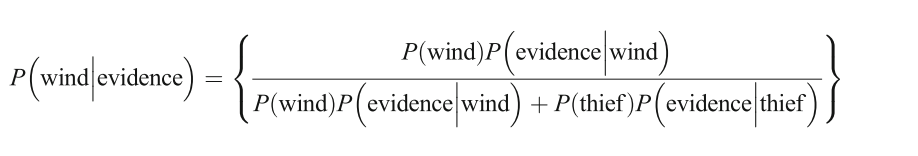
\includegraphics[scale=.7]{images/windThief.jpeg}
      \caption{Bayesian model for the prediction of wind as the cause of the window creaking, see Pezzulo (2013)}
        \label{fig:windThief}
   \end{center}
\end{figure}


\begin{enumerate}
  \item $P(wind)$: the model prior formulated by previous experience (e.g., it has been windy at night recently, or in the case of $P(thief)$, there have been some recent thefts in the neighbourhood)
  \item $P(evidence|wind)$: the likelihood that the sensory experience is caused by the wind (this value could be informed by other sources of information, e.g., the trees outside are also rustling, the dog is not barking (which may be the case if it were a thief, ($P(evidence|thief)$))
  \item Precision: the reliability or certainty associated with your sensory inputs (it is dark in your room and so you may not trust your visual perception, you just woke up so could have been dreaming, etc.).  The precision weight is factored into the ``evidence.''
\end{enumerate}

These hypotheses (wind and thief) effectively compete on the basis of how well they explain the sensory stimuli.  The brain's capacity to quantify the uncertainty of any given sensory state facilitates optimal selection between competing predictions pertaining to the same bottom-up sensory signals, judged probabilistically.  At any one moment, an individual has access to multiple hypotheses derived from priors, which compete for the best fit of the sensation, until that process leads to fixation on the best hypothesis for the sensory state.  Binocular rivalry, (for example looking at a necker cube) is an instance in which there is insufficient sensory information available in order to reach fixation on one model over another (see Figure ~\ref{fig:neckerCube} \citep{Frith2007}.  In the wind vs. thief example, based on the the priors ($P(wind) = .8$ (it has been windy recently) and $P(thief) = .2$ (no recent reports of theft)), and the (precision-weighted) evidence ($P(evidence|wind) = .6$ and $P(evidence|wind) = .5$ (roughly equivalent because it is dark and you have just woken up), the probability of wind ($= .8276$) is much higher than the probability of thief ($= .1724$).  In this case, the prediction that wind caused the window to creak wins out, and guides action and perception accordingly.

\begin{figure}[htbp]
  \begin{center}
    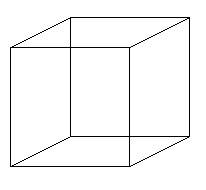
\includegraphics[scale=.7]{images/Necker_cube.png}
      \caption{Necker Cube: Binocular rivalry is due to insufficient sensory information to reach fixation on one explanatory model over another}
        \label{fig:neckerCube}
   \end{center}
\end{figure}

Original models of predictive coding dealt primarily with ``exteroceptive'' information \citep[relating to stimuli that are external to an organism, i.e. visual, auditory, haptic perception][]{Rao1999,Friston2010}.  For example, in the wind vs. thief model considered above, only exteroceptive evidence is considered, in the form of the auditory stimulus of the window creaking.  Research has since demonstrated that the predictive coding approach can also account for ``proprioceptive'' information (relating to stimuli that are produced and perceived within an organism, especially those connected with the position and movement of the body), as well as ``interoceptive'' information (relating to stimuli produced within an organism, particularly by the body's organs (viscera) e.g., heart rate, ``gut feelings,'' and so on).  Incorporating proprioceptive and interoceptive information sources into predictive processes allows researchers to theoretically demonstrate that human cognition is both ``embodied'' \citep[inference is rooted in and contingent upon visceral, interoceptive information ][]{Pezzulo2014}, and ``active'' \citep[in the sense that humans can move throughout the environment to reduce the discrepancy between proprioceptive predictions and actual body states][]{Friston2010,Clark2015}.
  \footnote{In the case of motor systems, agents are able to move their sensors in ways that amount to actively seeking or generating the sensory consequences that they (or rather, their predictive models) expect.  In this way, ``error signals self-suppress, not through neuronally mediated effects, but by eliciting movements that change bottom-up proprioceptive and sensory input''  \citep[][1349]{Friston2003}.}
The key point here is that the hierarchical and nonlinear structure of predictive coding enables diverse sensory inputs feed into the same inferential mechanism.  Diverse functions of action, cognition and perception are thus integrated into an framework that is both embodied and enactive \citep{Friston2015}.

Embodied and active sources of information in human cognition broaden the scope of human cognition beyond the brain, by reducing reliance upon computationally intensive mental simulation.  Instead, canny utilisation of extra-neural and bio-external affordances of the environment can support free energy minimisation \citep{Clark2015}.  Consider an embodied and active revision of the wind vs. thief example.  Two key differences in the model become apparent.  First, the evidence considered is broadened to include both interoceptive and proprioceptive cognitions.  Assume that before you went to bed you just watched a horror movie, and when you woke up to the sound of a window creaking your heart began to pound and you immediately fixated on the explanation that a thief was causing your window to creak.  Fixation on the thief hypothesis can be explained by the contribution of interoceptive information (e.g., autonomic stress response, heart beat, etc.) to sensory the evidence \citep{Pezzulo2014}.  In addition, the incorporation of proprioceptive information into the model (for example, the possibility of moving to turn on the bed-side lamp) creates additional cognitive affordances through which higher level predictions could be strengthened.  Even if turning on the light would subsequently reveal that it was the wind all along, this example shows how perception, emotion, and action are functionally integrated in human cognition.

Second, broadening sensory inputs in the model also introduces the problem of differential reliability of sensory inputs.  The wind vs. thief example describes a situation in which exteroceptive information is relatively unreliable: it is dark so visual inputs are restricted, and what you heard is unreliable because you just woke up and maybe it was part of a dream.  By contrast, in most cases, and particularly in this case, interoceptive information is quite certain: you can be certain that your heart is pounding and that you feel unnerved.  In this particular case, interoceptive inputs may have a greater influence on the overall inference.  Evidence suggests that the brain deals with multiple sensory inputs via a process of ``Bayesian multisensory integration'' \citep{Ernst2004}, with the reliability of each sensory input proportional to the inverse of its variance.  In the wind vs. thief example, the interoceptive information from your body, precision-weighted as the most reliable source, will likely tip the model to favour the hypothesis that it is a thief, in which case you will move your body in ways that reconcile discrepancy between proprioceptive predictions that also correspond to the thief hypothesis (i.e., instructing you to turn on the light) \citep{Pezzulo2014}.

In sum, active inference \citep[and the predictive coding paradigm which it extends, see][]{Clark2013} proposes a radical inverse of traditional models of cognition that rely predominantly on bottom-up sensory inputs and top-down feature detection \citep{Marr1985}. Instead, active inference posits that top-down predictive models themselves shape perception and action, and the only information that travels forward (or from the ``bottom-up'') is the error signals that arise from discrepancies between predictions and the sensorium \citep{Pickering2014}.  The active inference approach depicts a human cognitive system in which perception, mental simulation, emotion, and action are functionally and temporally integrated to manage uncertainty inherent in interactions with the environment \citep{Clark2013}.  In the next section, I explain how active inference can be applied to joint action and the phenomenon of team click.

%[; for a detailed discussion of the differences between traditional and active inference approaches to motor control, see Appendix ~\ref{app2:theory} Section  ~\ref{app2:motorControl}]

\subsection{Active inference in joint action \label{sect:activeInfJA}}

The active inference approach promises a testable theory of the embodied and dynamic dimensions of joint action that are captured by the phenomenology of team click.  As explained above, these dimensions of experience have been hitherto out of reach of traditional theoretical models, which have struggled to integrate cognition and emotion, mental simulation and habitual response, flexibility and efficiency in human cognition \citep{Clark2015}.

\subsubsection{Auxiliary Forward Model approach to joint action}
Attempts have been made to theorise joint action using conventional auxiliary models of cognition and action.  Keller and colleagues (2016), for example, presented a conceptual framework that applies AFM approach to musical joint actions.  The authors suggest that ensemble music making, such as a string quartet, requires three types of internal models: 1) self-internal models responsible for action planning and motor control, 2) other-internal models that support the prediction of other’s actions, and 3) joint-internal models, which keep a dynamic representation of the shared goal \citep{Keller2016}.  Of these three types of models, only self-internal models comprise the auxiliary predictive architecture (e.g., ``inverse models'' that output motor commands and ``efference copies'' of one’s own actions as forward models, see Appendix ~\ref{app2:theory}, Section ~\ref{app2:motorControl} for a more detailed explanation of these terms).  Each member of the quartet has different self-internal models of the notes played by their own instrument, and will have expectations about the notes that they hear from other instruments and the overall sound of the joint performance.  ``Compensatory control'' (the ability to correct deviations from the shared goal) is achieved by updating self-inverse models using the error signal obtained from comparing the actual joint state and the joint desired state; ``anticipatory control'' (the ability to execute actions based on predictions) is achieved by an adaptation signal that results from the comparison between predicted joint state and the desired joint state.

The proposal that individuals in joint action only produce auxiliary predictive models of their own actions serves to explain how individuals are able to preemptively attenuate sensitivity to their own action in order to attend to the actions (and prediction errors) of others.  This approach can also effectively explain the phenomenon of tickling, and particularly why it is near impossible to tickle oneself \citep[due to sensory attenuation resulting from the self-generated predictions about the consequences of action][]{Blakemore2003}

Pesquita and colleagues (2017) identify three shortcomings of this application of auxiliary forward models (AFM) to joint action.  First, the AFM approach does not explain how prediction error feedback reaches and updates model of the shared goal.  This issue limits the ability of AFM to account for the embodied and enactive dimensions of joint action, such as the flexibility of joint goals in joint action (e.g., switching between the shared goal of carrying a table or the bench depending on the location of both objects).  Second, the AFM approach lacks an mechanism that allows sensory feedback to reach the other-internal model. In the model proposed by Keller and colleagues, error signals are fed-back only to the self-inverse model, as no inverse model for the joint action partner exists. This missing link suggests the practical possibility that self and other models may gradually diverge over time \citep{Pickering2014}.  Third, Keller et al.’s proposal does not specify how sensory input is differentially used to update self and other models, which limits the model's ability to account for learning and adaptation within joint action \citep{Pesquita2017}.  Thus, not only does the AFM approach appear to be computationally intensive (due to the recruitment of auxiliary inverse models and dual motor commands), it also appears to be unable to fully account for the completeness and flexibility of real-world joint action.

As Wolpert (a proponent of the AFM approach) himself points out, movement is a complex process. Because there are often several solutions that may lead to the desired outcome, the information available for selection is often distorted and delayed (due to neural-muscular limitations), and the external environment is dynamic \citep{Wolpert1997}. Without an obvious solution to the shortcomings mentioned above, it is difficult to apply the AFM approach concretely to a large number of real-world social interactions where actors do not subscribe to the same interaction end-goal, which is often instead open-ended and multifaceted \citep{Pesquita2017}.

\subsubsection{Integrated forward model approach to joint action}
The active inference approach offers an alternative model for joint action that promises to more fully account for its cognitive, perceptual, and emotional complexity.  This account of joint action begins with the proposal that joint action entails two (or more) Bayesian predictive brains committed to modelling each other in order to minimise free energy \citep{Friston2015,Friston2015a}. In order to achieve free energy minimisation, the sensory stimuli produced by co-actors in joint action must be pre-emptively modelled, just like other features of the sensorium.  This necessitates a scenario in which brain A has a model of brain B, which includes the fact brain B is modelling brain A, and so on---\textit{ad infinitum}.  The recurrent predictions of both brains about one another threatens an infinite runaway regress that could preclude accurate modelling of either brain.  As Friston and Frith demonstrate formally, however, this recursion mathematically dissolves if the models of the two brains are formally similar \citep{Friston2015}.  If grounded in computational similarity, owing functionally equivalent models for joint action, each brain is able to generate predictions of the sensory outcomes caused by itself and the other in the same way.  The authors propose that this will lead to dynamical ``generalised synchronisation'' \citep{Barreto2003} between the internal models of both brains, such that they will be able to accurately predict each other's behaviour based on feedback of exteroceptive (sensory information from the actions of others and the task environment) and proprioceptive (pertaining one's own contribution to joint action) prediction errors.

In place of auxiliary processes of prediction, the active inference account of joint action hinges instead on the function of precision weighting of prediction errors in order to facilitate and finesse joint action.  When performing action, the an individual must turn down the volume (reduce the precision weighting) on prediction errors relating to one's own action so that movement can occur unimpeded by over-attention to self-generated prediction errors \citep[an intuitive example of the opposite of this ideal scenario is when the flow of speech is interrupted due to the availability of exteroceptive auditory feedback in the case of a Skype call][]{Friston2015}. Alternatively, when attending the the action of others in joint action, precision weighting is used to flexibly adjust the volume of multi-modal prediction errors (exteroceptive, interoceptive, and proprioceptive) in order to finesse and sustain generalised synchronisation (the shared narrative on which joint action is sustained).  Heuristically, this suggests that active inference presents in one of two modes; either 1) attending to sensations or
2) acting during periods of sensory attenuation \citep{Friston2015}.  The active inference explanation for ticklishness, for example, does not rely on auxiliary production of efference copies (or lack thereof).  Rather, ticklishness resembles the behavioural product of a mode of active inference in which the volume (precision weight) on proprioceptive prediction errors is ``dialled-up'' to the max.
  \footnote{Recall also that instances of tickling commonly involve a stationary victim. While it indeed appears almost impossible to tickle oneself, it is also rare to be tickled while moving, i.e., acting during periods of sensory attenuation.}

The radical proposal of the active inference approach to joint action is that, unlike the AFM approach, the AI approach formally theorises the way in which cognitive resources are shared between two or more brains, bodies, and the task-specific environment \citep{Clark2015}.
This ``shared narrative'' which supposedly transcends agency, is supported by the self-organising


\subsubsection{Predictive Joint Action Model (PJAM)}
Pesquita and colleagues \textcite{Pesquita2017} have formulated a minimal architecture for an active inference approach to joint action, which they term a ``Predictive Joint Action Model'' (PJAM).  PJAM is comprised of three hierarchical levels of inference: goal representation, action-planning, and sensory routing (see figure ~\ref{fig:PJAM}).  Each level of the hierarchical model is informed by prediction errors from the level below, and the model works iteratively to minimise free energy in joint action scenarios.  In line with the AI approach, PJAM does away with auxiliary processes of motor control and efferent copies, and posits instead that joint action emerges directly from two or more individuals reaching generalised synchronisation by converging on equivalent predictive models for joint action \citep{Friston2015}.

\begin{figure}[htbp]
  \begin{center}
    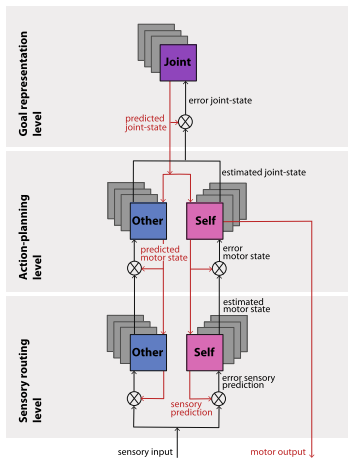
\includegraphics[scale=.8]{images/PJAM.png}
      \caption{The Predictive Joint Action Model \citep{Pesquita2017}}
        \label{fig:PJAM}
   \end{center}
\end{figure}

PJAM assumes that each participant in a joint-action maintains internal models of 1) the joint task, 2) the action contributions of self and others to the joint task, and  3) the sensory-motor inputs expected from action plans.

The \textit{goal-representation} level of PJAM suggests that participants in joint action generate and monitor representations of the shared task. This proposal is formulated from evidence that musicians maintain shared representation of desired unified sound of an ensemble \citep{Keller2008}.  In one study, for example, Loehr and colleagues  use a neurophysiological measurement that codes unexpected events (ERP) to show that musicians tracked deviations from a desired joint state \citep{Loehr2013}; in another study, Loehr and Vesper \textcite{Loehr2016} demonstrated that playing music together generates shared expectations regarding the desired state of joint action, and this process guides future action.  Taken together, this evidence suggests that participants in joint action utilise prediction errors arising from lower levels to update representations of shared tasks.  The key point here is that joint action is facilitated by embodied and inactive predictions of a shared task, and not just auxiliary predictions about an individual's role in shared processes, as an AFM approach would suggest \citep{Keller2016}.
%(Wolpert MOSAIC model doesn't account for updating rep. of shared task)

At the \textit{action-planning} level of PJAM, pairs of models predict the contributions of self and others to a joint action.  The ``shared narrative'' at the goal representation level generates discrete action plans for self and other, which are then tested against prediction errors arising from the sensory routing models below \citep{Pesquita2017}.  This level of PJAM is supported by evidence that participants in joint action generate internal models of self and other, known as co-representation, either spontaneously and involuntarily, as in the commonly used social simon task experimental paradigm \citep{Sebanz2003,Atmaca2008}, or more deliberately, as in a coordinated dyadic horizontal jumping task \citep{Vesper2012}.

Action-planning entails, on the highest level, action roles; on a mid-level, movement trajectories; and on the lowest level, movement of muscle groups of self and others \citep{Pesquita2017}.  As with goal representation, action-planning for self and others is a predictive process \citep{Flanagan2003}, in which individuals encode motor predictions and resulting errors of others' actions in addition to their own \citep{VanSchie2004,Radke2011}.  Predictive models of self and other action plans appear to be grounded in an individual's own motor simulation processes, such that each participant maintains covert motor activations relating to expected contributions of their partners \citep{Hollander2012}.

There is evidence to suggest that motor simulation of self and other action plans is mediated by the existence of a shared goal between co-actors \citep{Kourtis2010}.  Loehr and Vesper \textcite{Loehr2016} demonstrate that when learning a joint piano piece, musicians are able to better perform the piece together rather than solo, which suggests that representations about each participant in joint action are encoded within the joint context of the interaction.  In other words, when we learn a joint task we not only learn our own role, but also the impact of other's roles on our own role in the joint action.

In sum, the action planning level of PJAM proposes that models of the self and models of partners can be paired to represent the possible combinations of individual contributions to the joint action. These models transform the desired joint-state signal, descending from the goal representation level, into expectations of the unique motor states of the self and the partner.  Error signals arrive from levels of the model below, with sensory routing.  Studies also show that co-representation is modulated by mood \citep[positive or negative affect, see][]{Kuhbandner2010}, self-concept and social orientation \citep{Colzato2012,Colzato2012a}, and group membership \citep{DeBruijn2008,Iani2013}.

The \textit{sensory routing} level receives the inflow of sensory input and compares it to internal model predictions pertaining to each participant's action outcomes on the level above.  This comparison process serves as a gate for parsing sensory information into their corresponding predictive streams (self or others, see Figure ~\ref{fig:PJAM}). This process allows the predictive system to attribute external consequences to each individual’s actions.   For example, two people carrying a table will receive haptic input from the table. This input will be confounded with respect to its source, in that the haptic input itself does not differentiate between the forces that each brother applies to the table. However, the comparison between the haptic input and the separate predictions about one’s own and the other’s action will help feed each predictive cascade of self and other into their respective streams \citep{Pesquita2017}.

Consistent with other levels of PJAM, deviations between sensory input and sensory predictions (i.e., prediction errors) are fed-back to sensory predictive models in order to continuously improve sensory parsing.  As foreshadowed above, evidence indicates that accurate prediction of others' actions is associated with the attenuation of sensorial experience of joint action outcomes.  Predictions about motor outcomes are used to filter out the sensory feedback produced by the same action \citep{Blakemore1999}.  This proposal is confirmed by evidence that greater sensorial experience occurs when an outcome is unexpected, as opposed to predicted from prior self or other action \citep{Sato2008}.  In addition, attributing sensory consequences to joint action partners is linked to cooperative success \citep{Chaminade2012}, suggesting that finely tuned sensory routing based on predictions of self and other actions could be key to successful coordination.

In real world joint action scenarios such as interaction team sport, co-actors interact and rehearse their behaviours to produce a hierarchy of aligned representations, an implicit common ground on which joint action can unfold \citep{Noy2017}.  PJAM provides a framework for the function of active inference in processes of alignment and movement coordination.  Each level of PJAM generates predictions of the information that it expects to be found on the level below.  Continuous comparison between adjacent levels results in error signals that are fed back to optimise subsequent predictions in the level above.  This hierarchical predictive architecture for joint action allows humans to generate accurate yet flexible models for joint action.


\subsubsection{A continuum of solutions to joint action}

The explanatory power of PJAM (and the active inference approach more generally) lies in its capacity to incorporate various cognitive strategies within one overarching mandate of free energy minimisation \citep{Clark2015}.  The distinction between cortical and extra-cortical, mental and emotional, model-based and model-free cognitive processes collapsed under an approach in which a continuum of cognitive strategies are flexibly deployed to exploit brain, body, and bio-external resources \citep{Pezzulo2013}.  Bayesian optimisation facilitates this flexibility: the volume on sensory prediction error signals is either dialled up or dialled down depending on their experience-based reliability (inverse of variance of the prior distribution).  As such, just as the binary distinction between mental and emotional collapses, so too does the distinction between external and internal, exteroceptive and interoceptive (and proprioceptive) \citep{Seth2013}.

Evidence discussed below suggests that optimal solutions to joint action confined to scenarios like group exercise may tend to favour the recruitment of more extra-neural resources as a way of minimising free energy, whereas less efficient solutions to joint action may rely on more computationally intensive procedures in order to reduce free energy.

\subsubsection{Direct coupling deriving from general synchronisation in joint action}

An active inference approach to joint action is grounded in thermodynamic cognition and dynamical systems theory \citep{Friston2013}.  Friston and Frith point out that generalised synchronisation---what they call the ``shared narrative'' that enables joint action---is an inevitable and emergent property of coupling two systems that are trying to predict each other ~\ref{Friston2015}.  Generalised synchrony refers to the synchronisation of chaotic dynamics \citep{Barreto2004}.  The basic principle is as follows.  If the universe comprised two biological (free energy minimising) systems---you and me---then your states and my states have to be restricted to an attracting set of states that is small relative to all possible states we could be in \citep{Friston2015}.  This attracting set of states enforces a generalised synchrony in the sense that the state you are in imposes constraints on states I occupy.  It is in this sense that generalised synchronisation is a fundamental aspect of coupled dynamical systems that are free energy minimising.  Furthermore, if we are both trying to minimise the free energy of our attracting set (by reducing surprise or entropy), then synchronisation will be more manifest \citep{Friston2015a}.

The relevant prediction that follows from this theory is that joint action will exhibit properties of dynamical systems, namely, coupling of system component degrees of freedom \citep{Turvey1978,Schmidt1990}.  Dynamic coupling can be identified by two core properties:  1) dimensional compression (potentially independent DF are coupled so that the synergy possesses a lower dimensionality than the set of components from which it arises) and 2) reciprocal compensation (the ability of one component of a synergy to react to changes in others) \citep{Riley2011}.  Indeed, an accumulation of evidence has identified the existence of functional synergies on multiple levels of behaviour, from brain function \citep{Yufik1998,Sengupta2013}, to interpersonal interactions \citep{Kelso2009,Riley2011,Fusaroli2014}, to large-scale human societal dynamics \citep{Nowak2017}.

In the case of joint action in particular, individuals have been found to couple and reciprocally constrain their movements reducing the overall control needed to maintain effective cooperation \citep{Ramenzoni2011,Ramenzoni2012,Riley2011,Schmidt1990}.  Individuals’ behaviours become increasingly interdependent, so that a higher-level structure of the interaction emerges. This kind of emerging organisation has previously been referred to as soft-assembly \citep{Kello2009}: individuals preserve a degree of autonomy, but their behaviour is constrained by the interaction. They can flexibly engage and disengage from it, as well as become part of other soft-assemblies \citep{DeJaegher2010,DiPaolo2012}.

Research into the coordination dynamics of real-world joint actions  has shown evidence of dynamic coupling in joint-action tasks, such as dancing, martial arts, and moving objects like furniture.  In these studies, specific component degrees of freedom are modelled as coupled oscillators \citep[using the HKB model, which describes the change in the relative phase between two oscillatory components.   See][]{Haken1985,Kelso1986}.  Models are analysed for non-random fluctuations in relative phase over multiple time scales.  This type of synchronisation is said to be of a fractal or semi-fractal organisation, also known as 1/f scaling or ``pink noise'' \citep{Caron2017}. According to Anderson and colleagues \citep{Anderson2012}, 1⁄f scaling is ubiquitous in smooth cognitive activity, and indicates a self-similar structure in the fluctuations that occur over time (within a time series of measurements).
1⁄f scaling indicates that the connections among the cognitive system's components are highly nonlinear \citep{Ding2002,Holden2013,Kello2010,Riley2011,VanOrden2003,VanOrden2005}. Interestingly, pink noise has been measured beyond dyadic synchronisation, in the analysis of sub-phases of team sports \citep{Passos2014,Duarte2012} and group dancing \citep{Chauvigne2017}.
  \footnote{1⁄f scaling is temporal long-range dependencies in the fluctuations of a repeatedly measured behaviour or activity. Analogous to spatial fractals, 1⁄f scaling denotes a fractal or self-similar structure in the fluctuations that occur over time. That is, higher frequency, lower amplitude fluctuations are nested within lower frequency, higher amplitude fluctuations as one moves from finer to courser grains of analysis \cites(for a more detailed description see, for example)(){Holden2005}{Kello2009}.}

In addition to the pink noise of dynamic coupling in joint action, research has also attempted capture movement signatures of joint action that resemble instances of ``identical synchronisation'' or  being ``in the zone'' with a co-actor.  Working within the common dyadic ``mirror game'' paradigm, Noy and colleagues \textcite{Noy2011,Noy2015,Hart2014} have developed an experimental proxy for an optimal state of togetherness in joint action.  ``Co-confident motion'' (CC motion) is canonical movement pattern of synchronised motion characterised by smooth and jitter-less motion, without the typical jitter resulting from reactive control in more commonly encountered leader-follower patterns.  In CC motion, different players appear to shift their basic motion signatures to a movement shape that is altogether different from their individually preferred shapes \citep{Hart2014}. Importantly, the pattern of CC motion shares the same sine wave shape as the optimal solution of the minimum jerk model, a well-known motor control model for rhythmic motion \citep{Hogan2007}.

Noy and colleagues suggest that it is possible that during CC motion periods of joint action, two players converge to a canonical pattern stemming from an optimal state of each participant’s motor control system.  The resulting motion may be easier to predict and to agree on. Furthermore, participants appear to use smooth elementary strokes of CC motion as the building blocks for more complex motion \citep{Noy2017}.  This observation raises the possibility that CC motion, a state of alignment in which individual components converge in a transcendent, functional synergy, could set the cognitive foundation for more efficient and effective higher level processes of communication and information transfer \citep[15]{Lerique2016}.  This evidence accords with the proposal that joint action is underwritten by the fact that two or more agents share functionally and formally equivalent ``shared narrative'' that transcend self and other agency, and instead involve a ``we'' mode of social cognition \citep{Gallotti2013}.

In support of this line of research, experimental evidence has shown that functional interpersonal synergies (dynamic coupling) facilitate performance of social cognitive or linguistic tasks, such as gaze coordination and turn taking in conversation \citep{Miles2010,Richardson2005,Shockley2009}.  Conversely, being psychologically distanced from another individual can inhibit the emergence of interpersonal synergies \citep{Miles2010}.  The ways in which functional interpersonal synergies facilitate adaptive information transfer between individuals and within groups suggests that psychological mechanisms and cultural practices responsible for generating these synergies could have been subject to cultural evolutionary forces of selection and attraction \citep{Claidiere2014,Mesoudi2016a}.


%The notion of generalised synchrony may also lend a formal backdrop to observations of synchronisation of brain activity between agents during shared perspective taking Moll & Meltzoff, 2011). For example, functional magnetic resonance imaging, suggests that internal action simulation synchronises action–observation networks across individuals (Nummenmaa et al., 2014).



\subsubsection{Active reinterpretation of action perception links}
Evidence of dynamic coupling between co-actors in joint action is further bolstered by parallel strands of research in psychology \citep{Prinz1990,Prinz1997,Prinz2013}, neurophysiology \citep{Rizzolatti2004,Rizzolatti2010}, and neurocognition \citep{Wolpert1998,Wolpert2000} that interpersonal behavioural coordination in joint action is facilitated by the intrinsic coupling—--under certain circumstances---of action perception and action execution in the human brain.

Since Prinz’s (1990) initial proposal that perception and action are coded in a common representational domain, and are therefore linked by shared neural resources, research into action-perception coupling has spanned individual action as well as interpersonal social interaction.
In terms of its function for joint action scenarios, action-perception coupling is regarded as a basic link between sender and receiver \citep{Rizzolatti1998} that provides procedural, perceptual, and emotional common ground between individuals.

In essence, action-perception coupling refers to the ostensive co-occurrence of a stimulus for action and its motor representation.  For example, the representation of a perceptual effect (say the sound of a middle-C on a piano) can trigger the movement necessary to produce the effect itself (motor instructions for playing the middle-C key on a piano).   Importantly, evidence suggests that sensory-motor coupling emerges primarily as a result of motor learning: having only visual \citep{Candidi2014} or auditory \citep{Lahav2007} experience with a given action is not sufficient to trigger these motor responses—--active motor learning is necessary.  As such, most research into action-perception coupling occurs with individuals who have mastered a certain sensorimotor task, such as expert musicians, whose movements and intended sounds become strongly associated \citep{Novembre2014}.

In behavioural experiments in which samples of musicians are compared to non-musician controls, researchers demonstrate that auditory perception primes action if strong action-perception links have been established through instrument-specific training \citep{Drost2005,Drost2005a,Drost2007}.  For example, Drost and colleagues showed that sound cues incongruent with the prescribed action response (the sound cue of a D chord when the prescribed action response is a C chord) delayed execution time \citep{Drost2005} and induced more false responses \citep[i.e., production of the heard chord, instead of the imperative one,][]{Drost2005a} in pianists but not non-pianists.  Keller and Koch \textcite{Keller2006} showed that mental images of anticipated action effects can prime responses to a similar degree as is observed with congruent and incongruent sounds, highlighting the role of action-perception coupling in action preplanning (i.e., before sounds are actually perceived).  Further studies demonstrated that action-perception coupling does not only enhance the efficiency of action planning, but also facilitates timing accuracy and economical force control by optimising movement kinematics \citep{Keller2010}.

Neurophysiological evidence suggests a neural signature for action-perception coupling in the motor cortices.  Haueisen and Knosche \citep{Haueisen2001} conducted a magnetoencephalography (MEG) study (of piano players with and without experience) and showed that perception of piano pieces led to an increase of neural activity over the motor cortex hand area in piano players but not non-musicians.  Bangert and colleagues \textcite{Bangert2006} ran an fMRI study where professional pianists and non-musicians heard novel piano sequences that were synthesised online (and therefore could not be familiar).  Compared to non-musicians, professional pianists showed a broad network of motor areas responding to the piano sequences, including both primary motor and premotor (BA 4/6) regions.  Besides auditory- and visual-motor coupling, tactile, proprioceptive and haptic sensory feedback has been shown to induce coupling \citep{Schulz2003,Kuchenbuch2014}.

These behavioural and neurophysiological data, taken together, indicate that musical training leads to the emergence of cross-modal action-perception coupling, where perception of the effects of musical actions (either the sounds produced or the visual presentation of the movement patterns) triggers proprioceptive predictions for the movements necessary to produce these effects. Interestingly, these effects have also been observed in trained non-experts \citep{Bangert2003,Lahav2007}.  Lahav and colleagues (2007), for example, trained non-musicians to play a piano piece by ear (without notation) over a period of five days and found that activation of the frontoparietal motor-related network (comprising Broca’s area, the premotor region, the intraparietal sulcus, and the inferior parietal region) increased most strongly for the trained pieces, versus untrained (but motorically known) and familiar but motorically unknown pieces.

It has been argued that the function of action perception coupling is twofold.  First, coupling of this nature supports a neurophysiological capacity to anticipate (generate predictions about) our own as well as other's  (i.e., observed) actions.  Maidhof et al. \textcite{Maidhof2009} and Ruiz et al. \textcite{Ruiz2009} conducted two similar EEG studies in which they examined the ERPs preceding the execution of piano errors in pianists and non-musicians.  In pianists (but not non-musicians) errors were detected prior to their execution (the EEG signal was found to anticipate the actual mistake by 100 ms \citep{Maidhof2009} and 50–70 ms \citep{Ruiz009}.  These data thus indicate that the coupling of sensory and motor cortices has a strong anticipatory character that, given the existence of an association between movements and their ensuing effects, permits the generation of predictions about the state of our own body and the sensory consequences of our movements.

Second, action-perception links act as a resource for the co-representation of and coordination with others in joint action.
Research demonstrates that the training-mediated coupling of perception and action is not confined to individual behaviour.  As mentioned above, there is evidence to suggest that expert ensemble musicians form representations of self and other-related actions, and that these representations are influenced by properties of the individual’s own motor system \citep{Novembre2012}.  Action-perception links can be used for monitoring and integrating (e.g., timing or combined pitches) the actions of other ensemble members with self-generated actions \citep{Loehr2013}, and these effects appear to be stronger in individuals with high perspective taking skills \citep{Novembre2012,Loehr2013}.  The overlap between mechanisms for action production and action observation suggests that individuals may represent their own and others’ actions in a commensurable format.  Training-induced motoric representation of self and other actions may facilitate various capacities important for joint action, such as prediction, adaptation, and entrainment.

These various strands of research, when recast in an active inference paradigm, can be understood as evidence for the role of Bayesian precision-weighting of error-signals for the optimisation of performance in joint action.  Tight coupling between action and perception in expert practitioners indicates high precision weighting of interoceptive and proprioceptive prediction errors.   According to PJAM, tight coupling of perception and action is the result of an iterative learning process in which individuals develop a ``grasp'' of a 1) shared narrative for action, 2) predictions concerning the action plans of self and other, and 3) routing of exteroceptive, proprioceptive, and interoceptive prediction error signals.  In other words, this grasp in joint action is equivalent to the optimal reduction in free energy across multiple hierarchical layers of prediction in the brains of each co-actor.

%Explain with AFM is not the best model for explaining action-perception links


\subsection{Individual differences}

There is evidence to suggest that individual differences may impact upon joint action.  Research suggests that preexisting dispositional tendencies in sociality dimensions of personality (e.g. extroversion, agreeableness) and social orientation (locus of control, communication styles), as well as the nature of pre-existing interpersonal relationships, and technical competence in joint action \citep{Novembre2014}, will impact on the structure and quality of interpersonal movement coordination and, presumably, the social unity that emerges from joint action \citep{Marsh2009}.

The personality concept of empathy—understanding others’ thoughts and feelings—has been linked to anticipatory mechanisms related to action simulation \citep{Sevdalis2014,Keller2014}.  In the piano studies mentioned above \citep{Novembre2012}, scores on the ‘perspective-taking’ sub-scale of an empathy questionnaire correlated positively with neurophysiological measures of representing the other’s part in their own motor system, as well as how much this ‘other-representation’ was relied upon for coordination \citep{Novembre2014a}.  In a synchronised finger-tapping task, Pecenka and Keller (2011) found that scores on a perspective-taking questionnaire correlated with the degree that individuals predicted event micro-timing in a tempo-changing pacing sequence.  \textcite{Richardson2007} found in a dyadic plank moving experiment, individuals’ levels of agreeableness and extroversion were positively correlated with persistence of cooperation in the task.

Social orientation and motivation have also been shown to effect interpersonal coordination.  A study of unintentional coordination revealed that prosocial-oriented individuals spontaneously synchronised arm movements with others more than pro-self-oriented individuals, whether their social/self-orientation reflected their pre-existing disposition or resulted from an experimental manipulation \citep{Lumsden2012}.  Studies have found that interacting with a late-arriving partner reduced stepping synchronisation, compared with interacting with a partner who arrived on time \citep{Miles2010}, and bodily synchrony decreased during arguments compared with affiliative conversations Paxton2013.

A recent study addressed the relationship between locus of control (i.e. the degree to which life events are perceived to result from one’s own actions) and temporal adaptation (error correction) \citep{Fairhurst2014}.   Results indicated that individuals with an internal locus of control (who attribute the cause of events to their own actions) engaged in less phase correction than individuals with an external locus of control (who attribute events to external factors), which may reflect individual variation in predispositions towards different movement coordination strategies.  This assertion is corroborated by a study conducted by Schmidt and colleagues \textcite{Schmidt1994}, which used interpersonal wrist-pendulum coordination to investigate the effects of self-reported social competence \citep{Riggio1996} upon social coordination stability.  Subjects were selected to create homogeneous social competence dyads (High–High or Low–Low pairs) and heterogeneous dyads (High–Low pairs). The heterogeneous (High–Low) pairs demonstrated significantly greater stability and fewer breakdowns in coordination than the homogeneous (High–High and Low–Low) social competence pairings, suggesting that reciprocity (leader-follower) rather than symmetry (leader-leader or follower-follower) of social competence facilitates social coordination.  In this sense,  ``internal'' individuals may stabilise the tempo of their own performance (at the expense of synchrony) and take a leader role, whereas ``external'' individuals may synchronise with their partner (at the expense of maintaining a steady tempo) and take a follower role.  In sum,  dispositional tendencies movement coordination and in sociality dimensions might set the initial conditions that make pull to the cooperation attractor stronger (or weaker) than a pull to the autonomy attractor (independent action).

Autism/schizophrenia spectrum of individual variation...


  \subsection{Cultural affordances}

There is also evidence to suggest that informational affordances provided by the specific cultural milieu can serve to shape patterns of behaviour relevant to joint action. The term ``culture'' can be understood as shared elements that provide standards for perceiving, believing, evaluating, communicating, and acting among those who share a language, a historical period, and a geographical location \citep{Triandis1996}.  Alternatively, as cultural psychologists Kitayama and Markus (2020, p. 422) explain, culture is a:

\begin{quotation}
  ...stand-in for a similarly untidy and expansive set of material and symbolic concepts...that give form and direction to behaviour [and that] culture is located in the world, in patterns of ideas, practices, institutions, products, and artefacts.
\end{quotation}


The theory of affordances \citep{Gibson1979}, meanwhile, has been influential within and beyond cognitive psychology.  Affordance theory states that the world is perceived not only in terms of object shapes and spatial relationships but also in terms of object possibilities for action (affordances).  This definition accords neatly with the propositions of the active inference paradigm, which posits a circular causal loop between perception and action, mediated by cognitive resources distributed throughout brains, bodies, and physical features of the task-specific environment.

Within the active inference paradigm itself, Pezzulo suggests that an affordance is the attribute of a hidden cause in the environment that induces (through predictive coding) predictions in the exteroceptive and proprioceptive domains \citep[908]{Pezzulo2013}.  As Pezzulo explains:

    \begin{quotation}
    ...predictive coding hierarchies can go well beyond two or three levels and can combine heterogeneous elements at the different levels.  At the lowest levels, perceptual hypotheses that are close to the sensory and interoceptive events are considered; at the highest levels more profound regularities can be represented, and the hierarchy can include, at least in principle, long-term beliefs that are increasingly more removed from sensorimotor events and that are mainly acquired through cultural learning (but that still remain grounded through the linkage with lower-level events).
    \end{quotation}

In this sense, cultural affordances can be understood as regularities that cue multi-modal predictions for joint action.
These understandings of culture-as-affordances incorporates factors that are both psychologically explicit or ``external,'' such as societal values or similar cultural dimensions, (Hofstede1991,2001; Schwartz1992; SoaresFarhangmehrShoham2006), social practices (NisbettMasuda2003), and artefacts (CraigDouglas2006), as well as and ``internal,'' such as dominant modes of self-construal or dispositional and linguistic tendencies \citep{Markus1991}.

In the active inference account, cultural affordances can be understood as frames of reference act as ``hyper-priors'' that set the macro-contextual coordinates for joint action \citep{Clark2013}, or the ``common narrative'' that stabilises alignment of predictions \citep{Friston2015}.

Joint actions that involve complex sequences and divisions of labour between participants appear to rely heavily on capacities to explicitly signal intention for the assigning of roles, forward planning, and repair of failed coordination \citep{Frith2010}.  These ``coordination smoothers'' \citep{Vesper2017} often function to reduce spatial and temporal variation in action by providing a shared spatiotemporal referent for co-alignment of predictions.

Cultural conventions are thus examples of effective framing devices for joint action.  Depending on the context of the joint action, it could be subject to a pre-existing, mutually recognised power relations typical in the established culture (e.g., favouring hierarchical or egalitarian communication, \citep[see]{Cheon2011}) and the particular situational context (e.g., formal or informal).  Establishing roles, such as leader or follower, also has a similar smoothing effect, and often the affordances in the task environment shape the smoothing strategies available to co-actors \citep{Marsh2009}.

Contextual (cultural) affordances for joint action appear to be dictated by processes operating at multiple conceptual levels---from the micro-level predictive processes associated with movement action and perception, to the macro-level predictive frames offered by specific cultural and contextual niches---interact in complex processes of reciprocal causation to shape joint action.  Conceptualisation of the causal complexity of cognitive processes relevant to joint action in this way echoes a broader reconceptualisation of the causal complexity associated with change on an evolutionary timescale, which recognises that human behavioural phenomena is the result of a number of biological, cognitive, and ecological mechanisms that interact via reciprocal feedback loops spanning varying scales of time and space \citep{Fuentes2015}.

A key insight overlooked by the existing social high account of group exercise and social cohesion, but revealed by the paradigm shift surrounding active inference, is the sensitivity of joint action (or any cognitive process for that matter) to informational affordances provided by various layers of ecological and cultural context.


\subsection{Summary of the active inference approach to joint action}






\section{Active inference in group exercise \label{sect:activeInfGE}}



Active inference under conditions of high uncertainty
- in the moment; on-line
- physiological exertion

The issue of research only on dyadic situations:
  What about scenarios involving many actors?

  Group exercise contexts create an environment in which cortical processing power is strained.

physical exertion leads to down-regulation of cortical structures could lead to increased attenuation of proprioceptive prediction errors. (Neurocog evidence to support).



\subsection{More efficient joint action relies on more on direct coupling?}

The thermodynamic mandate of free energy minimisation predicts a tendency towards more efficient solutions to the challenges of joint action, without compromising task-specific function.  While interoceptive predictive models are flexible and effective for the purposes of establishing and maintaining coordination in joint action, they do come at a (computational) cost.  The thermodynamic approach to joint action predicts that more efficient and effective joint action will recruit mechanisms and strategies that outsource the computational cost of joint action to sources beyond the brain. In the case of highly skilled practitioners, whose interoceptive predictive models are presumably highly attuned to the affordances of the task environment, it is plausible that extra-neural and even extra-personal resources could provide a more cognitively efficient and effective route to the performance of successful joint action.  In which case, it is possible that the tacit and sub-perceptual quality of ``team click'' in joint action could be indirect phenomenological evidence of optimal movement coordination.

Interestingly, studies of highly skilled practitioners in joint action demonstrate that more technically competent practitioners generate more accurate predictive models for joint action than less technically competent practitioners \citep{Tomeo2012,Aglioti2008,Mulligan2016}.   In studies involving skilled versus non-skilled practitioners in dyadic interactions, it has been shown that more skilled practitioners create stronger dynamical coupling through flexibly modulating their actions with others \citep{Schmidt2011, Caron2017}. These findings are corroborated by other studies that find that professional footballers (versus novice controls) are able to more accurately predict the direction of a kick from another player's body kinematics (\cite{Tomeo2012}, see also \cite{Aglioti2008,Mulligan2016} for similar results with basketball and dart players).

Interestingly, when analysing co-regulation between members of basketball teams, it was shown by Bourbousson \textcite{Bourbousson2015} that more expert teams made fewer mutual adjustments (at the level of the activity that was meaningful for co-actors), suggesting an enhanced capability of expert social systems to achieve and maintain an optimal level of awareness during the unfolding activity, potentially implicating down-regulation of prediction error management processes, and greater reliance on extra-neural couplings with co-actors and the physical environment.

A recent field study by R'Kiouak and colleagues (2016) supported this line of reasoning.  Through combined analysis of phenomenological and video data derived from a close study of two unacquainted expert rowers who participated in a real world dyadic rowing exercise (coxless pair), the authors found that athletes reported joint action as being salient and meaningful only 24.5\% of the race under study (e.g., during synchronisation breakdowns), whereas the rowers did not pay attention to the effectiveness of their joint action for the remaining 75.5\% of the studied period \citep{RKiouak2016}.  In other words, these results suggest that the rowers were able to coordinate their strokes through experiencing their joint action as meaningless during a large part of their crew activity.  These results lead the authors to suggest that extra-personal regulation processes might have underlain the dynamics of the joint action, such that athletes used the environment to mediate/organise the arrangement of individual activities. This corroborates that team coordination patterns of movement may occur without a perfectly shared experience about the ongoing joint action \citep{Bourbousson2011,Bourbousson2012}. The study provides evidence that the full coordination of sense-making activities is not needed to allow for a viable patterned joint action in a natural task, as long as actors are simultaneously involved in co-regulating their collective behaviour (Froese and Di Paolo, 2011; Froese et al., 2014a,b).  The authors interpret the results as evidence for a stigmergic theory of collective behaviour (Susi and Ziemke, 2001; Avvenuti et al., 2013), in which holistic phenomena of coordination might be considered as emerging from the behaviour–environment coupling.

The prevalence of evidence describing action-perception linkages and extra-neural direct coupling with intra- and extra-personal resources of the task specific environment in joint action scenarios involving highly skilled practitioners suggests a tendency towards less computationally expensive mechanisms of joint action and an overall reduction in free energy in the coordination environment.  This evidence suggests that team click could be phenomenological evidence of a mode of interpersonal coordination in joint action that is less reliant on higher order interoceptive action-oriented modelling, and more dependent on lower-cognitive mechanisms of movement regulation.


\subsection{Social connection through joint action}






























\section{A novel theory of social bonding through joint action}

\subsection{Perceptions of success in joint action predict team click}

Team click predicts social bonding: Social connection through joint action\label{sect:DVsocialBonding}

The link between interpersonal coordination and social bonding has been addressed in the behavioural mimicry and synchrony literatures \citep[e.g.,][]{Wheatley2012,Launay2016,Mogan2017}, but there is less substantive evidence in relation to dynamic interpersonal coordination in natural joint action settings such as those found in group exercise contexts \citep{Marsh2009,Miles2009,Lumsden2012}.  There is strong evidence from the synchrony literature to suggest that a combination of 1) neuropharmacological reward arising from lower-cognitive affective mechanisms, 2) self-other merging resulting from neurocognitive alignment, and 3) reinforcement of cooperative relationships owing to experience of interpersonal alignment in joint action generates a psychophysiological environment conducive to generating social bonds.  As discussed above, successful joint action in humans requires a continuum of strategies ranging from interoceptive predictive modelling (of the shared task as well as the action plans of self and others required for the shared task), to direct coupling with the task-specific environment via the recruitment of lower-cognitive mechanisms of movement regulation \citep[e.g., proprioceptive mechanisms of balance and orientation][]{Semin2008} .  Precisely which strategies (and in which scenarios these strategies) could be responsible for social connection in joint action remains poorly understood.

\subsubsection{Affect}
The affective consequences of joint action appear to be an important source of information for social cognitions between co-actors.  Observation and anecdote in sport, for example, suggest that part of the exhilarating nature of team click is the way in which the experience of joint action induces positively valenced surprise resulting from a violation of athletes' prior expectations regarding the outcome of joint action \citep{Jackson1999}.  Likewise, unsuccessful joint action appears to induce an inverse, negatively valenced violation of expectations, linked to emotional states of displeasure \citep{Ekkekakis2003}.  The experience of positive surprise in joint action appears to be linked to a attribution of collective (over personal) agency \cite{Sato2005,Sato2008}, and the experience of negative surprise in joint action meanwhile appears linked to feelings of personal guilt and shortcomings vis-a-vis the group \citep{Kenworthy2011,Mckimmie2015}.  Therefore, it is quite possible that processes of prediction error management and minimisation associated with joint action oriented predictive models could be an important source of information for social cognitions relevant to social bonding.

Emotion in the ``active inference'' paradigm of social cognition is best conceptualised as a superordinate program (or series of programs) for adaptive organismic regulation, whereby emotion functions as a feedback signal informing future behaviour \citep{Cosmides2000,Chetverikov2014,Chetverikov2015,Barrett2017}.  The original distinction in cognitive science between cognition and emotion was supported by the idea that segregated brain areas implement cognitive and emotional functions and that there are two independent processing routes, one cognitive/controlled and one emotional/automatic, which usually compete (but also occasionally cooperate) to control behaviour \citep{Kahneman2003}.  However useful this ``dual-systems'' view has been thus far in cognitive science, prevailing evidence concerning the complexity of functional integration and segregation of brain processes challenges the cognitive-emotional distinction \citep{Pessoa2013}.  The emerging view is not only that cognition interacts with emotion at many levels, but that in many respects they are functionally integrated and continuously impact each other's processing.

Cortical processes of prediction error management appear to be mediated by the activity of the dopaminergic system \citep{Schultz2016}, while subcortical neuromodulatory systems, such as those responsible for producing norepinephrine, acetylcholine, and endogenous opioids, appear to be involved in attuning cortical processing to signals from the body and environment that are important for survival \citep{Lewis2005}.  There is now evidence to suggest that complex cognitive processes (traditionally understood to be confined to cortical regions) and subcortical neuromodulatory systems (traditionally understood to be responsible only for affective response and exogenous to the brain's inferential processes) work in a loop of reciprocal interaction in order to enhance processes of error management \citep{Damasio1994,Lewis2005,Miller2017,Barrett2017}.
%Emotions can in this sense be understood more as superordinate programs for regulating disparate subordinate cognitive modules for the purposes of global coordination with the environment \citep{Cosmides2000}.  Collapsing the common neurocognitive distinction between cortical and subcortical processes helps integrate the role of affective processes in active inference and their downstream social effects.


Chetverikov \textcite{Chetverikov2016} and colleagues have suggested a model for explaining the function of ``surprise'' in joint action.  In line with prevailing understandings of emotion in cognition, authors propose that affect serves as feedback on predictions, reflecting their accuracy and regulating them so that confirmed predictions are more likely to be used again \citep{Chetverikov2014}.  Furthermore, if predictions are confirmed (low prediction error), feedback is weighted with inverse prior probabilities of predictions, so that more probable predictions receive less positive feedback. In other words, confirmation of more probable predictions yields \textit{less} positive feedback than confirmed less probable predictions.  This model allows for the prediction that more positive violations of expectations in joint action will produce stronger affective feedback.

\subsubsection{Agency}
In addition to the affective consequences of joint action, there is evidence to suggest that perceptions of agency may also be important in a relationship between joint action and social bonding. Generally speaking, the successful matching of action predictions with sensory outcomes is thought to correspond to the experience of agency, which refers to the perception of causing something to happen by intention \citep{Frith2007,Pacherie2012,Obhi2011}.  It remains unclear, however, whether or how processes of prediction error management, which appear to be largely pre-perceptual, are related to the conscious experience of agency \citep{Pesquita2017}.

It is plausible to assume that, within a predictive coding model of cognition, a sense of agency would be achieved through a match between higher level intentional action planning, and corresponding sensory effects at a lower level \citep{VanderWel2012}.  It is now a well established fact that participants in joint action are able to attenuate or cancel sensory inputs from their own contributions to joint action if these inputs have already been predicted as part of interoceptive models \citep{Blakemore2005}.  Because an individual's own movement in joint action is directly predicted, its sensory consequences can be perceptually attenuated relative to external sensations without compromising the ongoing interaction \citep{Blakemore1999}. One popular example of sensory cancellation is the observation that it is hard, if not impossible, to tickle oneself: the prediction of the sensory consequences of tickling dampens the sensory experience of the tickling itself \citep{Frith2007}.  Evidence suggests that interpersonal sensory cancellation occurs in an analogous way when our predictions of someone else’s actions dampen the sensorial experience of these outcomes\citep{Sato2008}.  This research suggests that the alignment of hierarchical predictions and sensory input produces stable personal agency in joint action.

By contrast, discrepancy between prediction and sensory input can alter the experience of agency \citep{Sato2008}.  Unpredicted sensory input can lead to ascribing agency for that input to an external source, for example, other participants in joint action or the external environment \citep{Sato2005,Frith2007}.  As has been well documented in the case of schizophrenia, attribution of agency in social interaction may be modulated by individual variation in ``locus of control'' (the degree to which events are perceived to result from one’s own actions or not), and this may be related to improper function of the parietal cortex \citep{Frith2000}. In healthy adult populations of humans, meanwhile, it can be predicted that ascribing agency to sources external to the self will occur more in situations in which the discrepancy between predicted and actual sensory input is at its larger.  Presumably, according to Chetverikov's model connecting prediction and affect at least, the more a sensory input violates existing predictions, the more salient these experiences will be, and the more likely they will arouse the need for attributions of causal agency at the conscious level of experience \citep{Pesquita2017}.

The link between interpersonal coordination and social bonding has been addressed in the behavioural mimicry and synchrony literatures \citep[e.g.,][]{Wheatley2012,Launay2016,Mogan2017}, but there is less substantive evidence in relation to dynamic interpersonal coordination in natural joint action settings such as those found in group exercise contexts \citep{Marsh2009,Miles2009,Lumsden2012}.  More recently, however, analysis of dynamic coupling of co-actors in joint action scenarios reveals that synchronised movement implicates an array of implicit and pre-perceptual cognitive processes of alignment and prediction error minimisation \citep{Schmidt2011}, which, in addition to more explicit forms of communication, could be central to the generation of feelings of self-other merging, self-other distinction, and perceived reliability and trust associated with social bonding \citep{Marsh2009}.

A recent study used a finger tapping paradigm (in which participants coordinated taps with a virtual partner prone to drift in tap tempo) to address the relationship between locus of control and temporal adaptation (error correction) \citep{Fairhurst2014}.  Individuals with an internal locus of control (who attribute the cause of events to their own actions) engaged in less phase correction than individuals with an external locus of control (who attribute events to external factors). This result indicates that individual variation may lead to certain default patterns of interpersonal movement coordination (such the default leader-follower dynamic).



\subsection{Higher levels of team click predict higher levels of social bonding}

The components of team click outlined above indicate that this often observed phenomenon contains elements of positive expectation violation deriving from an experience of tacit or implicit coordination in joint action.  This phenomenology suggests that the joint action could entail the perception of unexpected, i.e., action that was not simulated by explicit regions of the predictive architecture of joint action.  Team Click could be a mode of movement coordination that relies heavily, or at least in part, in extra-neural mechanisms of dynamic coupling.  Not only is team click often not explicitly predicted (in which case the experience of team click could lead to ascribing agency of joint action to co-actors or to another ``mysterious'' source).

At the same time, not only is team click a phenomenon largely outside a normal participant's locus of control, it is also highly improbably, even if practitioners are co-familiar and aligned.  Team click in real world settings requires orchestration and coordination of multiple joint tasks across multiple sensory modalities.
According to the affect-prediction model, the fact that team click is such a highly improbable occurrence means that the affective charge of this occurrence should also be high \citep{Chetverikov2016}.  In this way, the improbability and unpredictability of team click could activate both 1) high levels of affect and 2) a social target for this affective response.  The fact that team click appears to maximise an interaction between affect and agency make it a perfect candidate for a psychological phenomenon capable of the relationship between joint action and social bonding.


%attributing sensory consequences to joint action partners is linked to cooperative success Chaminade2012, potentially via the parietal operculum (Goodbody and Wolpert 1998)


\subsection{Team click will mediate a direct relationship between joint action and social bonding in group exercise}






\section{Predictions of the theory}


    The overarching prediction of this thesis is that the psychological phenomenon of team click mediates a relationship between joint action and social bonding.

    Within this main hypothesis, I also formulate the following sub-hypotheses:
    \begin{enumerate}
      \item Athletes who perceive greater success in joint action will experience higher levels of felt ``team click.'' I predict that relevant perceptions of joint action success will relate to athlete perceptions of:
        \begin{enumerate}
          \item a combination of specific technical components; or
          \item an overall perception of team performance relative to prior expectations; or
          \item an interaction between these two dimensions of team performance.
        \end{enumerate}
      \item Athletes who experience higher levels of team click will report higher levels of social bonding.
      \item More positive perceptions of joint action success will predict higher levels of social bonding, driven by more positive:
      \begin{enumerate}
        \item perceptions of components of team performance;; or
        \item violation of team performance expectations; or
        \item an interaction between these two predictors.
      \end{enumerate}
    \end{enumerate}



Individual differences



Culture






\subsection{A novel approach to joint action and social bonding}

Current evidence suggests the possibility that, in general, more coordinated human movement systems place less demands on cognitively expensive mechanisms of predictive action-oriented motor simulation, and instead rely more on lower cognitive mechanisms of movement regulation that facilitate more direct coupling between the organism and the affordances of the physical environment \citep{Bourbousson2011,RKiouak2016}.  Establishing self-organising functional interpersonal synergies allows for individuals to outsource more of the cognitive demands of joint action to extra-neural mechanisms of free-energy minimisation \citep{Clark2013}.

This generalisable tendency in human movement systems towards thermodynamic efficiency may also be a source of the social bonding effects of joint action.  If optimal coordination in joint action tends to entail greater down-regulation of higher order (more abstract) cortical processes of prediction \citep{Dietrich2004b}, then the subsequent subjective experience of optimal coordination should involve an element of surprise due a participant's relative lack of perceptual anticipation of the outcome.  Research from the social cognition of joint action suggests that participants attribute causal agency for unanticipated outcomes more commonly to social actors rather than to the self \citep{Sato2008}.  Moreover, less anticipated outcomes in joint action also appear to produce a higher affective response, such that more desirable but less probable predictions produce more positive affective feedback \citep{Chetverikov2016}.  The combination of these two mechanisms may explain why the phenomenology of team click mediates a relationship between joint action and social bonding.  Team click is surprising, emotionally rewarding, and readily attributed to the agency of others---the combination of these ingredients creates a strong foundation for social affiliation between co-participants in joint action.


\section{Chapter overview}


                                              \end{CJK}{UTF8}{gbsn}
